\documentclass[aspectratio=169,11pt]{beamer}

% Moloch (maintained Metropolis successor) with Purdue colors.
\usetheme[progressbar=frametitle, sectionpage=progressbar, numbering=fraction]{moloch}
\definecolor{PurdueBlack}{HTML}{000000}
\definecolor{PurdueGold}{HTML}{CFB991}
\definecolor{PurdueRush}{HTML}{DAAA00}
\definecolor{PurdueAged}{HTML}{8E6F3E}
\definecolor{PurdueSteel}{HTML}{555960}
\definecolor{PurdueDust}{HTML}{EBD99F}
\definecolor{LecBlue}{HTML}{0969DA}
\setbeamercolor{normal text}{fg=black!90, bg=white}
\setbeamercolor{frametitle}{fg=white, bg=PurdueBlack}
\setbeamercolor{progress bar}{fg=PurdueRush, bg=PurdueDust}
\setbeamercolor{title separator}{fg=PurdueRush}
\setbeamercolor{progress bar in section page}{fg=PurdueRush, bg=PurdueDust}
\setbeamercolor{alerted text}{fg=PurdueAged}
\setbeamercolor{example text}{fg=LecBlue}
\setbeamercolor{block title}{fg=black, bg=PurdueDust!70}
\setbeamercolor{block body}{bg=PurdueDust!20}

\usepackage{amsmath,amssymb,mathtools,bm}
\usepackage{booktabs}
\usepackage{tikz}
\usetikzlibrary{positioning,calc,arrows.meta,backgrounds,fit}
\usepackage{pgfplots}
\pgfplotsset{compat=1.18}
\usepgfplotslibrary{fillbetween}
\usepackage{listings}
\lstset{basicstyle=\ttfamily\scriptsize, columns=fullflexible, keepspaces=true,
  backgroundcolor=\color{PurdueDust!25}, frame=none, breaklines=true}

% Generated by scripts/make_lecture_data.py; do not edit by hand.
\newcommand{\EightMaxScore}{378}
\newcommand{\EightMinScore}{160}
\newcommand{\EightRuntime}{45}
\newcommand{\GameLL}{3,202 / -39}
\newcommand{\GameLLserved}{A 100\,MW, B 43.2\,MW}
\newcommand{\GameLS}{351 / 1,601}
\newcommand{\GameNashText}{Nash equilibrium: (A small, B small).}
\newcommand{\GameSL}{1,601 / 351}
\newcommand{\GameSS}{1,601 / 1,601}
\newcommand{\HCabove}{148}
\newcommand{\HCbuses}{2,000}
\newcommand{\HCmedian}{379}
\newcommand{\HCmin}{10}
\newcommand{\HCpninety}{1,543}
\newcommand{\HCpoints}{8,000}
\newcommand{\HCpten}{134}
\newcommand{\HCruntime}{8,000 LPs}
\newcommand{\OrdBus}{7419}
\newcommand{\OrdForty}{354}
\newcommand{\OrdFortyGain}{27}
\newcommand{\OrdTen}{303}
\newcommand{\OrdTenGain}{9}
\newcommand{\OrdZero}{278}
\newcommand{\PairHCa}{123}
\newcommand{\PairHCaGiven}{82}
\newcommand{\PairHCb}{136}
\newcommand{\SerOneBus}{1002}
\newcommand{\SerOneMed}{126}
\newcommand{\SerOneMin}{124}
\newcommand{\SerTwoBus}{7419}
\newcommand{\SerTwoMed}{502}
\newcommand{\SerTwoMin}{278}
\newcommand{\StoB}{200}
\newcommand{\StoBig}{392}
\newcommand{\StoBus}{7419}
\newcommand{\StoHalfNo}{278}
\newcommand{\StoHalfWith}{312}
\newcommand{\StoMean}{392}
\newcommand{\StoMin}{278}
\newcommand{\StoP}{50}
\newcommand{\StoWith}{312}


\newcommand{\HC}{\ensuremath{\mathrm{HC}}}
\newcommand{\MW}{\ensuremath{\,\mathrm{MW}}}
\newcommand{\MWh}{\ensuremath{\,\mathrm{MWh}}}
\newcommand{\src}[1]{{\scriptsize\color{PurdueSteel}[#1]}}

\title{Hosting Capacity and the Data-Center Connection Game}
\subtitle{How much load can a bus take, and who gets it?}
\author{Minghao Mou}
\institute{Elmore Family School of Electrical and Computer Engineering, Purdue University}
\date{Guest lecture, October 2026}

\begin{document}

\maketitle

% ===========================================================================
\begin{frame}{Why this question, now}
  \begin{itemize}
    \item Large new loads, especially AI data centers, ask for hundreds of MW at
      one point of the transmission grid.
    \item Before a request is approved, the utility must answer:
      \alert{how much load can this bus take without violating network limits?}
    \item When several requests compete for the same headroom:
      \alert{who gets served, and how much?}
  \end{itemize}
  \vspace{0.6em}
  \textbf{Today}
  \begin{enumerate}
    \item Hosting capacity as an optimization problem: one bus, many periods,
      many buses, with local generation and storage, with flexibility.
    \item The connection game: a classroom version of this planning problem on a
      2{,}000-bus synthetic Texas grid.
  \end{enumerate}
\end{frame}

% ===========================================================================
\section{Hosting capacity}

\begin{frame}{What is hosting capacity?}
  \begin{block}{Definition}
    The largest amount of new generation or \emph{load} that can be connected
    without performance becoming unacceptable, with the existing network and
    controls.
    \src{Bollen \& Hassan 2011; Bollen \& R\"onnberg 2017}
  \end{block}
  \begin{itemize}
    \item EPRI: ``the amount of PV that can be accommodated without impacting
      power quality or reliability under existing control and infrastructure
      configurations'' \src{Rylander et al., EPRI 2015}
    \item Originally for PV on distribution feeders; the same idea applies to
      large loads on transmission \src{Cicilio et al. 2021; Wan et al. 2026}.
    \item Ways to compute it: stochastic (Monte Carlo), streamlined, time-series,
      and \alert{optimization-based} \src{Mulenga et al. 2020; Ismael et al. 2019}.
  \end{itemize}
\end{frame}

\begin{frame}{Single-bus load hosting capacity as an LP}
  Extra load $L$ at bus $k$ in period $t$; existing generators redispatch:
  \begin{align*}
    \HC_{k,t} = \max_{L,\,p,\,\theta} \quad & L\\
    \text{s.t.}\quad
    & \textstyle\sum_{g\in\mathcal G_n} p_g + s_{n,t} - d_{n,t} - L\,\mathbf{1}[n=k]
      = \sum_{\ell:\,o(\ell)=n} f_\ell - \sum_{\ell:\,r(\ell)=n} f_\ell \quad \forall n\\
    & f_\ell = b_\ell(\theta_{o(\ell)} - \theta_{r(\ell)}),\quad |f_\ell| \le F_\ell
      \quad \forall \ell\\
    & p_g^{\min} \le p_g \le p_g^{\max}\quad \forall g,\qquad \theta_{\mathrm{ref}} = 0,\quad L\ge 0
  \end{align*}
  \begin{itemize}
    \item The DCOPF constraints with one extra load; the cost objective is
      replaced by ``make $L$ as large as possible'' \src{Alturki et al. 2018; Wan et al. 2026}.
    \item At the optimum a line or the generation limit binds: the
      \alert{bottleneck} of bus $k$ (read off the duals).
    \item PTDF view: $|f_\ell(L)| = |f^0_\ell - \mathrm{PTDF}_{\ell,k}L + \dots| \le F_\ell$,
      so buses ``far'' from tight lines host more.
  \end{itemize}
\end{frame}

\begin{frame}{Hosting capacity varies a lot across buses}
  \begin{columns}[T,onlytextwidth]
    \begin{column}{0.55\textwidth}
      \begin{tikzpicture}
        \begin{axis}[width=0.9\linewidth, height=5.4cm, ybar, bar width=4pt,
          xlabel={$\min_t \HC_{k,t}$ on the peak day (MW)}, ylabel={buses},
          ymin=0, xmin=0, axis lines*=left, tick label style={font=\scriptsize},
          label style={font=\scriptsize}]
          \addplot[fill=PurdueGold, draw=PurdueAged] table[x=bin_mw, y=count, col sep=comma]{data/hc_histogram.csv};
        \end{axis}
      \end{tikzpicture}
    \end{column}
    \begin{column}{0.42\textwidth}
      \small
      ACTIVSg2000, 2028 Jul--Dec, peak-load day (four 6-hour periods),
      all \HCbuses{} buses:
      \begin{itemize}
        \item median \HCmedian\MW
        \item 10\% of buses below \HCpten\MW
        \item 90\% of buses below \HCpninety\MW; \HCabove{} buses above 2{,}000\MW{} (not shown)
        \item smallest: \HCmin\MW
      \end{itemize}
      \vspace{0.3em}
      Computed with the course tool
      \texttt{ercot-game-hosting-capacity} (Gurobi, \HCruntime).
    \end{column}
  \end{columns}
\end{frame}

\begin{frame}{Over time: the stressed periods bind}
  \begin{columns}[T,onlytextwidth]
    \begin{column}{0.58\textwidth}
      \begin{tikzpicture}
        \begin{axis}[width=0.9\linewidth, height=5.2cm, xlabel={6-hour period of 2028 Jul--Dec},
          ylabel={$\HC_{k,t}$ (MW)}, axis lines*=left, legend style={font=\scriptsize, draw=none, at={(0.98,0.98)}, anchor=north east},
          tick label style={font=\scriptsize}, label style={font=\scriptsize}, xmin=0, xmax=736]
          \addplot[PurdueAged, thin] table[x=period, y=b7419, col sep=comma]{data/hc_series.csv};
          \addlegendentry{bus 7419}
          \addplot[LecBlue, thin] table[x=period, y=b1002, col sep=comma]{data/hc_series.csv};
          \addlegendentry{bus 1002}
        \end{axis}
      \end{tikzpicture}
    \end{column}
    \begin{column}{0.4\textwidth}
      \small
      A constant load must be served in \emph{every} period:
      \[
        \HC_k = \min_t \HC_{k,t}
      \]
      \begin{itemize}
        \item Bus \SerTwoBus: min \SerTwoMin, median \SerTwoMed\MW{}
          (load-driven: tight in peak periods)
        \item Bus \SerOneBus: min \SerOneMin, median \SerOneMed\MW{}
          (structural: almost constant)
      \end{itemize}
      ``Dynamic hosting capacity'' treats this time variation explicitly
      \src{de Oliveira et al. 2019}.
    \end{column}
  \end{columns}
\end{frame}

\begin{frame}{Many buses at once: the hosting-capacity region}
  \begin{columns}[T,onlytextwidth]
    \begin{column}{0.5\textwidth}
      \begin{tikzpicture}
        \begin{axis}[width=0.9\linewidth, height=5.4cm, xlabel={new load at bus 1002 (MW)},
          ylabel={new load at bus 1010 (MW)}, axis lines*=left, xmin=0, ymin=0,
          tick label style={font=\scriptsize}, label style={font=\scriptsize}]
          \addplot[name path=b, thick, PurdueAged] table[x=la, y=lb, col sep=comma]{data/pair_boundary.csv};
          \path[name path=axis] (axis cs:0,0) -- (axis cs:\PairHCa,0);
          \addplot[PurdueGold!60] fill between[of=b and axis];
          \draw[dashed, PurdueSteel] (axis cs:\PairHCa,0) |- (axis cs:0,\PairHCb);
          \node[font=\scriptsize, anchor=north east, align=right] at (axis cs:\PairHCa,\PairHCb) {box of\\single-bus HCs};
        \end{axis}
      \end{tikzpicture}
    \end{column}
    \begin{column}{0.48\textwidth}
      \small
      \[
        \begin{gathered}
          \mathcal H = \bigl\{x \ge 0 :\ \exists\,p_t \text{ feasible}\\
          \text{with loads } d_t + x\ \ \forall t\bigr\}
        \end{gathered}
      \]
      \begin{itemize}
        \item A convex polytope (projection of the DCOPF feasible set)
          \src{Gong \& Cobben 2024}.
        \item Single-bus HCs are its axis intercepts; they \alert{do not add up}
          \src{Wan et al. 2026}.
        \item Peak period: bus 1002 hosts \PairHCa\MW{} alone, but only
          \PairHCaGiven\MW{} once 60\MW{} sit at neighbor 1010.
      \end{itemize}
    \end{column}
  \end{columns}
\end{frame}

\begin{frame}{With a local generator}
  Site at bus $k$: load $L$, private generator $0\le g_t\le G$. The grid only
  sees the \emph{net} withdrawal $L-g_t$:
  \[
    \text{feasible} \iff \exists\, g_t\in[0,G]:\ L - g_t \le \HC_{k,t}\ \ \forall t
    \quad\Longrightarrow\quad \HC_k^{G} = \min_t \HC_{k,t} + G .
  \]
  \begin{itemize}
    \item Exact when the generator is always available; with outages, ramping,
      or fuel limits, $\HC^G_k \le \HC_k + G$.
    \item It runs only when the grid is short or when its cost
      ($\$80$--$250$/MWh in the game) is below the local price.
    \item Buying headroom: in the game \$1.5M per MW of generator, versus
      \$25M per MW of site that would otherwise go unserved.
  \end{itemize}
\end{frame}

\begin{frame}{With storage: periods become coupled}
  Battery at bus $k$: power $P$, energy $B$, signed output $p_t$
  (positive = discharge), period length $\Delta t$:
  \begin{align*}
    \HC_k^{S} = \max_{L,\,p,\,e}\ L \quad \text{s.t.}\quad
      & L - p_t \le \HC_{k,t}, \qquad -P \le p_t \le P,\\
      & e_t = e_{t-1} - \Delta t\, p_t,\qquad 0 \le e_t \le B,\qquad e_0 = e_T .
  \end{align*}
  \begin{itemize}
    \item A multi-period LP: the battery discharges in tight periods and must
      recharge in slack ones, using the same headroom.
    \item Summing over a cycle ($\sum_t p_t = 0$) gives
      $\HC^S_k \le \frac1T \sum_t \HC_{k,t}$: storage can at best lift the
      limit from the \emph{minimum} to the \emph{average} headroom.
    \item Power ($L \le \HC_{k,t} + P$) and energy (the running deficit must
      fit in the battery) keep it below that.
  \end{itemize}
  \src{Macedo et al. 2017 (storage to raise HC); general formulation}
\end{frame}

\begin{frame}{Storage in the game: one day, four 6-hour periods}
  \begin{columns}[T,onlytextwidth]
    \begin{column}{0.52\textwidth}
      \begin{tikzpicture}
        \begin{axis}[width=0.9\linewidth, height=5.0cm, ybar, bar width=12pt,
          symbolic x coords={1,2,3,4}, xtick=data, xlabel={period of the peak day},
          ylabel={MW}, ymin=0, axis lines*=left, enlarge x limits=0.2,
          legend style={font=\scriptsize, draw=none, at={(0.5,1.02)}, anchor=south, legend columns=3},
          tick label style={font=\scriptsize}, label style={font=\scriptsize}]
          \addplot[fill=PurdueGold, draw=PurdueAged] table[x=t, y=hc, col sep=comma]{data/storage_day.csv};
          \addlegendentry{$\HC_{k,t}$}
          \draw[thick, LecBlue] (axis cs:1,\StoMin) -- (axis cs:4,\StoMin)
            node[pos=0, anchor=north west, font=\tiny, text=LecBlue] {no battery};
          \draw[thick, dashed, PurdueAged] (axis cs:1,\StoWith) -- (axis cs:4,\StoWith)
            node[pos=0, anchor=south west, font=\tiny, text=PurdueAged] {with battery};
        \end{axis}
      \end{tikzpicture}
    \end{column}
    \begin{column}{0.46\textwidth}
      \small
      Game rules: $\Delta t = 6$\,h, $B = 4P$, each day starts and ends at
      $e = B/2$. Bus \StoBus, peak day:
      \begin{itemize}
        \item no battery: \textcolor{LecBlue}{\StoMin\MW}
        \item average headroom: \StoMean\MW{} (upper limit)
        \item with $P=\StoP\MW$, $B=\StoB\MWh$: \textcolor{PurdueAged}{\StoWith\MW}
      \end{itemize}
      A 6-hour period at full power would need $6P > B = 4P$\,MWh, so the
      \alert{energy} limit binds: even fully charged beforehand, the battery
      adds at most $B/\Delta t = \tfrac23 P$ in one tight period
      (here $+33\MW$). Over the half-year: \StoHalfNo{} $\to$ \StoHalfWith\MW.
    \end{column}
  \end{columns}
\end{frame}

\begin{frame}{Flexibility: curtail in a few periods}
  \begin{columns}[T,onlytextwidth]
    \begin{column}{0.52\textwidth}
      \begin{tikzpicture}
        \begin{axis}[width=0.9\linewidth, height=5.0cm, xlabel={$K$ = 6-hour periods that may be curtailed},
          ylabel={$\HC^{(K)}_{k}$ (MW)}, axis lines*=left, xmin=0,
          tick label style={font=\scriptsize}, label style={font=\scriptsize}]
          \addplot[thick, PurdueAged, mark=*, mark size=1.2pt] table[x=K, y=hc, col sep=comma]{data/order_statistic.csv};
        \end{axis}
      \end{tikzpicture}
    \end{column}
    \begin{column}{0.46\textwidth}
      \small
      Flexible connection \src{Gu, Chen \& Qin 2026}:
      \[
        \begin{aligned}
          \max_{C,u}\ & C\\
          \text{s.t.}\ & C + u_t \le \HC_{k,t},\quad u\le 0,\quad \|u\|_0 \le K
        \end{aligned}
      \]
      Nonconvex ($\|u\|_0$), but for one bus:
      \[
        \HC_k^{(K)} = \HC_{k,[K+1]},
      \]
      the $(K{+}1)$-th \emph{smallest} value. Bus \OrdBus: \OrdZero\MW{} at $K=0$,
      \OrdTen\MW{} at $K=10$ (60\,h, $+$\OrdTenGain\%), \OrdForty\MW{} at
      $K=40$ ($+$\OrdFortyGain\%). Diminishing returns in $K$; on a
      distribution feeder Gu et al.\ report $+78\%$ at 1\% of slots.
      See also \src{Etherden \& Bollen 2011; Sarker \& Dahlin 2026}.
    \end{column}
  \end{columns}
\end{frame}

\begin{frame}{How much should we trust a hosting-capacity number?}
  \begin{itemize}
    \item \textbf{Security.} Dropping N-1 contingencies overstates data-center HC
      by about 20\% on the IEEE RTS-24 \src{Wan et al. 2026}.
    \item \textbf{Dynamics.} The data center's own ride-through limits (UPS,
      converters) can be the binding constraint \src{Ren, Sun \& Teng 2026}.
    \item \textbf{Model.} DC power flow has no voltage or reactive-power limits
      and no losses.
    \item \textbf{Time resolution.} Averaging hours into longer periods smooths
      peaks and can overstate HC.
    \item \textbf{Simultaneity.} Single-bus numbers ignore everyone else who is
      connecting at the same time.
  \end{itemize}
  \vspace{0.3em}
  The last point is what the game is about.
\end{frame}

% ===========================================================================
\section{The connection game}

\begin{frame}{The game}
  \small
  \begin{columns}[T,onlytextwidth]
    \begin{column}{0.49\textwidth}
      \begin{itemize}
        \item Teams are data-center operators on ACTIVSg2000
          (2{,}000 buses, 3{,}206 branches).
        \item One CSV row per site: bus, connection $C$, generator $G\le C$,
          battery $P$ with $B=4P$.
      \end{itemize}
    \end{column}
    \begin{column}{0.49\textwidth}
      \begin{itemize}
        \item Six-hour periods (mean of 6 source hours), 4 per day,
          724--736 per half-year.
        \item The instructor solves one joint DCOPF with every team's sites.
      \end{itemize}
    \end{column}
  \end{columns}
  \vspace{0.6em}
  \centering
  \resizebox{0.84\textwidth}{!}{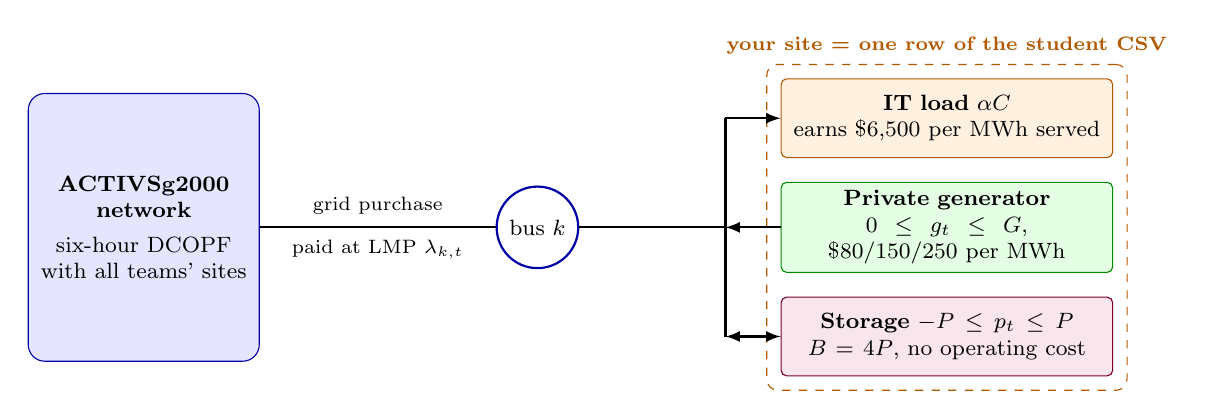
\begin{tikzpicture}[font=\footnotesize, >=latex]
  % Semantic anchors: ACTIVSg2000, student CSV, DCOPF, student preview.
  % One student CSV row attaches a site (load, private generator, storage) to one network bus.
  \tikzset{part/.style={draw, rounded corners=2pt, align=center, minimum height=10mm, text width=40mm, inner sep=3pt,
      execute at begin node={\hyphenpenalty=10000 }},
    load/.style={part, fill=orange!12, draw=orange!70!black},
    gen/.style={part, fill=green!10, draw=green!55!black},
    store/.style={part, fill=purple!10, draw=purple!65!black},
    grid/.style={draw=blue!65!black, fill=blue!10, rounded corners=6pt, align=center, minimum height=34mm, text width=27mm,
      execute at begin node={\hyphenpenalty=10000 }},
    link/.style={thick, draw=black}}
  \node[grid] (net) at (0,0) {{\bfseries ACTIVSg2000}\\{\bfseries network}\\[3pt]six-hour DCOPF with all teams' sites};
  \node[circle, draw=blue!65!black, fill=white, thick, minimum size=10mm, align=center] (bus) at (5.0,0) {bus $k$};
  \node[gen] (g) at (10.2,0) {{\bfseries Private generator}\\$0\le g_t\le G$, \$80/150/250 per MWh};
  \node[load, above=3mm of g] (it) {{\bfseries IT load} $\alpha C$\\earns \$6,500 per MWh served};
  \node[store, below=3mm of g] (s) {{\bfseries Storage} $-P\le p_t\le P$\\$B=4P$, no operating cost};
  \begin{scope}[on background layer]
    \node[draw=orange!70!black, dashed, rounded corners=4pt, fit=(it)(g)(s), inner sep=5pt,
      label={[font=\scriptsize\bfseries, text=orange!70!black]above:your site = one row of the student CSV}] (site) {};
  \end{scope}
  \draw[link] (net.east) -- node[above=1pt, font=\scriptsize] {grid purchase} node[below=1pt, font=\scriptsize] {paid at LMP $\lambda_{k,t}$} (bus.west);
  \coordinate (tap) at ($(g.west)+(-7mm,0)$);
  \draw[link] (bus.east) -- (tap);
  \draw[link] (tap |- it) -- (tap |- s);
  \draw[link, ->] (tap |- it) -- (it.west);
  \draw[link, <-] (tap) -- (g.west);
  \draw[link, <->] (tap |- s) -- (s.west);
\end{tikzpicture}
}
\end{frame}

\begin{frame}{Schedule and scoring}
  \small
  \begin{columns}[T,onlytextwidth]
    \begin{column}{0.46\textwidth}
      \begin{tabular}{@{}lll@{}}
        \toprule
        Week & Submissions & Counts?\\
        \midrule
        1 & 2027 Jan--Jun, Jul--Dec & practice\\
        2 & 2028 Jan--Jun, Jul--Dec & both\\
        3 & 2029 Jan--Jun, Jul--Dec & both\\
        \bottomrule
      \end{tabular}
      \vspace{0.6em}
      \begin{itemize}
        \item Sites built in Submission 1 stay for Submission 2 and are
          \alert{not charged again}.
        \item Submission 1 pays no energy cost.
      \end{itemize}
    \end{column}
    \begin{column}{0.52\textwidth}
      \centering
      score $=$ IT value $-$ energy $-$ gen.\ operating $-$ capital\\[0.5em]
      \footnotesize
      \begin{tabular}{@{}ll@{}}
        \toprule
        IT value & \$6{,}500 per MWh served\\
        energy & LMP $\times$ grid purchase\\
        generator operation & \$80 / 150 / 250 per MWh\\
        site & \$25M per MW\\
        generator capital & \$1.5M per MW\\
        storage capital & \$0.4M/MW $+$ \$0.25M/MWh\\
        \bottomrule
      \end{tabular}\\[0.6em]
      \begin{block}{Break-even share of load served}
        about 44\% over a week if built in Submission 1;\\
        87\% if added in Submission 2.
      \end{block}
    \end{column}
  \end{columns}
\end{frame}

\begin{frame}{The evaluator}
  \small
  For each day $d$ and period $t = 1,\dots,4$ ($\Delta t = 6$\,h): a DCOPF with
  all teams' sites, coupled through each battery's daily cycle.
  \begin{align*}
    \min\ & \textstyle\sum_{d,t} \Delta t \big(\sum_g c_g p_{g,dt} + \sum_s \sum_m c^m q^m_{s,dt}\big)\\
    \text{s.t.}\ & \text{DCOPF balance and line limits with loads } \alpha_i C_s
      \text{ and private } q_s, u_s\\
    & e_{s,d,t} = e_{s,d,t-1} - \Delta t\, u_{s,dt},\ \ 0\le e\le B_s,\ \ |u|\le P_s,\ \
      e_{s,d,0} = e_{s,d,4} = B_s/2\\
    & \textstyle\sum_{s\in i,\,k(s)=n} u_{s,dt} \le \sum_{s\in i,\,k(s)=n} \alpha_i C_s
      \quad\text{(a team's assets serve only its own load)}
  \end{align*}
  \begin{itemize}
    \item An exact LP that separates by day (Benders or one LP per day).
    \item LMP = dual of nodal balance; it prices energy in Submission 2.
  \end{itemize}
\end{frame}

\begin{frame}{When requests exceed the hosting-capacity region}
  \small
  The evaluator never uses first-come-first-served. It projects onto
  the region:
  \begin{enumerate}
    \item \textbf{Caps:} 100\MW{} per site, 500\MW{} per team, largest team
      capped at the smallest positive team request $\Rightarrow \hat d_i$.
    \item \textbf{Most service:} choose $\alpha_i\in[10^{-6},1]$ maximizing
      $\sum_i \alpha_i \hat d_i$ subject to joint feasibility in every period.
    \item \textbf{Proportional fairness} among near-optimal solutions
      \src{Kelly, Maulloo \& Tan 1998}:
      \[\textstyle \max \sum_i \log(\alpha_i \hat d_i).\]
  \end{enumerate}
  \begin{itemize}
    \item Capital is charged on what you \emph{asked} for, not on what is served.
    \item Alternatives worth discussing: first-come-first-served (today's
      interconnection queues), max--min fairness, prices
      \src{Liu et al. 2020; Gebbran et al. 2021}.
  \end{itemize}
\end{frame}

\begin{frame}{A two-team example on the real grid}
  \small
  Team A at bus 1002, team B at neighbor 1010; each picks 50 or 100\MW, built in
  Submission 1. Peak period, every period treated alike; payoffs per week (\$M):
  \vspace{0.3em}
  \begin{center}
    \begin{tabular}{@{}lcc@{}}
      \toprule
      A \textbackslash{} B & B small (50) & B large (100)\\
      \midrule
      A small (50) & \GameSS & \GameSL\\
      A large (100) & \GameLS & \GameLL\\
      \bottomrule
    \end{tabular}
  \end{center}
  \begin{itemize}
    \item One large, one small: infeasible; the caps cut the large request to
      50\MW, but it still pays for 100\MW.
    \item Both large: projection maximizes total service; the bus that uses less
      of the shared bottleneck is favored (\GameLLserved).
    \item \GameNashText
  \end{itemize}
\end{frame}

\begin{frame}[fragile]{What students get, and a live demo}
  \begin{columns}[T,onlytextwidth]
    \begin{column}{0.5\textwidth}
      \small
      \begin{itemize}
        \item \texttt{ercot-game-check-csv}: format and bus checks
        \item \texttt{ercot-game-preview}: approximate score, plan alone
        \item \texttt{ercot-game-hosting-capacity}: the LP from this lecture
        \item After each round: score breakdown, every team's $\alpha$,
          projection on/off, and a grid map
      \end{itemize}
      \vspace{0.3em}
\begin{lstlisting}
ercot-game-hosting-capacity \
  --artifact-dir .../2028/jul_dec \
  --start-period 304 --period-count 4 \
  --bus-id 1002 --bus-id 1010 \
  --output-dir demo/hc
\end{lstlisting}
    \end{column}
    \begin{column}{0.48\textwidth}
      \centering
      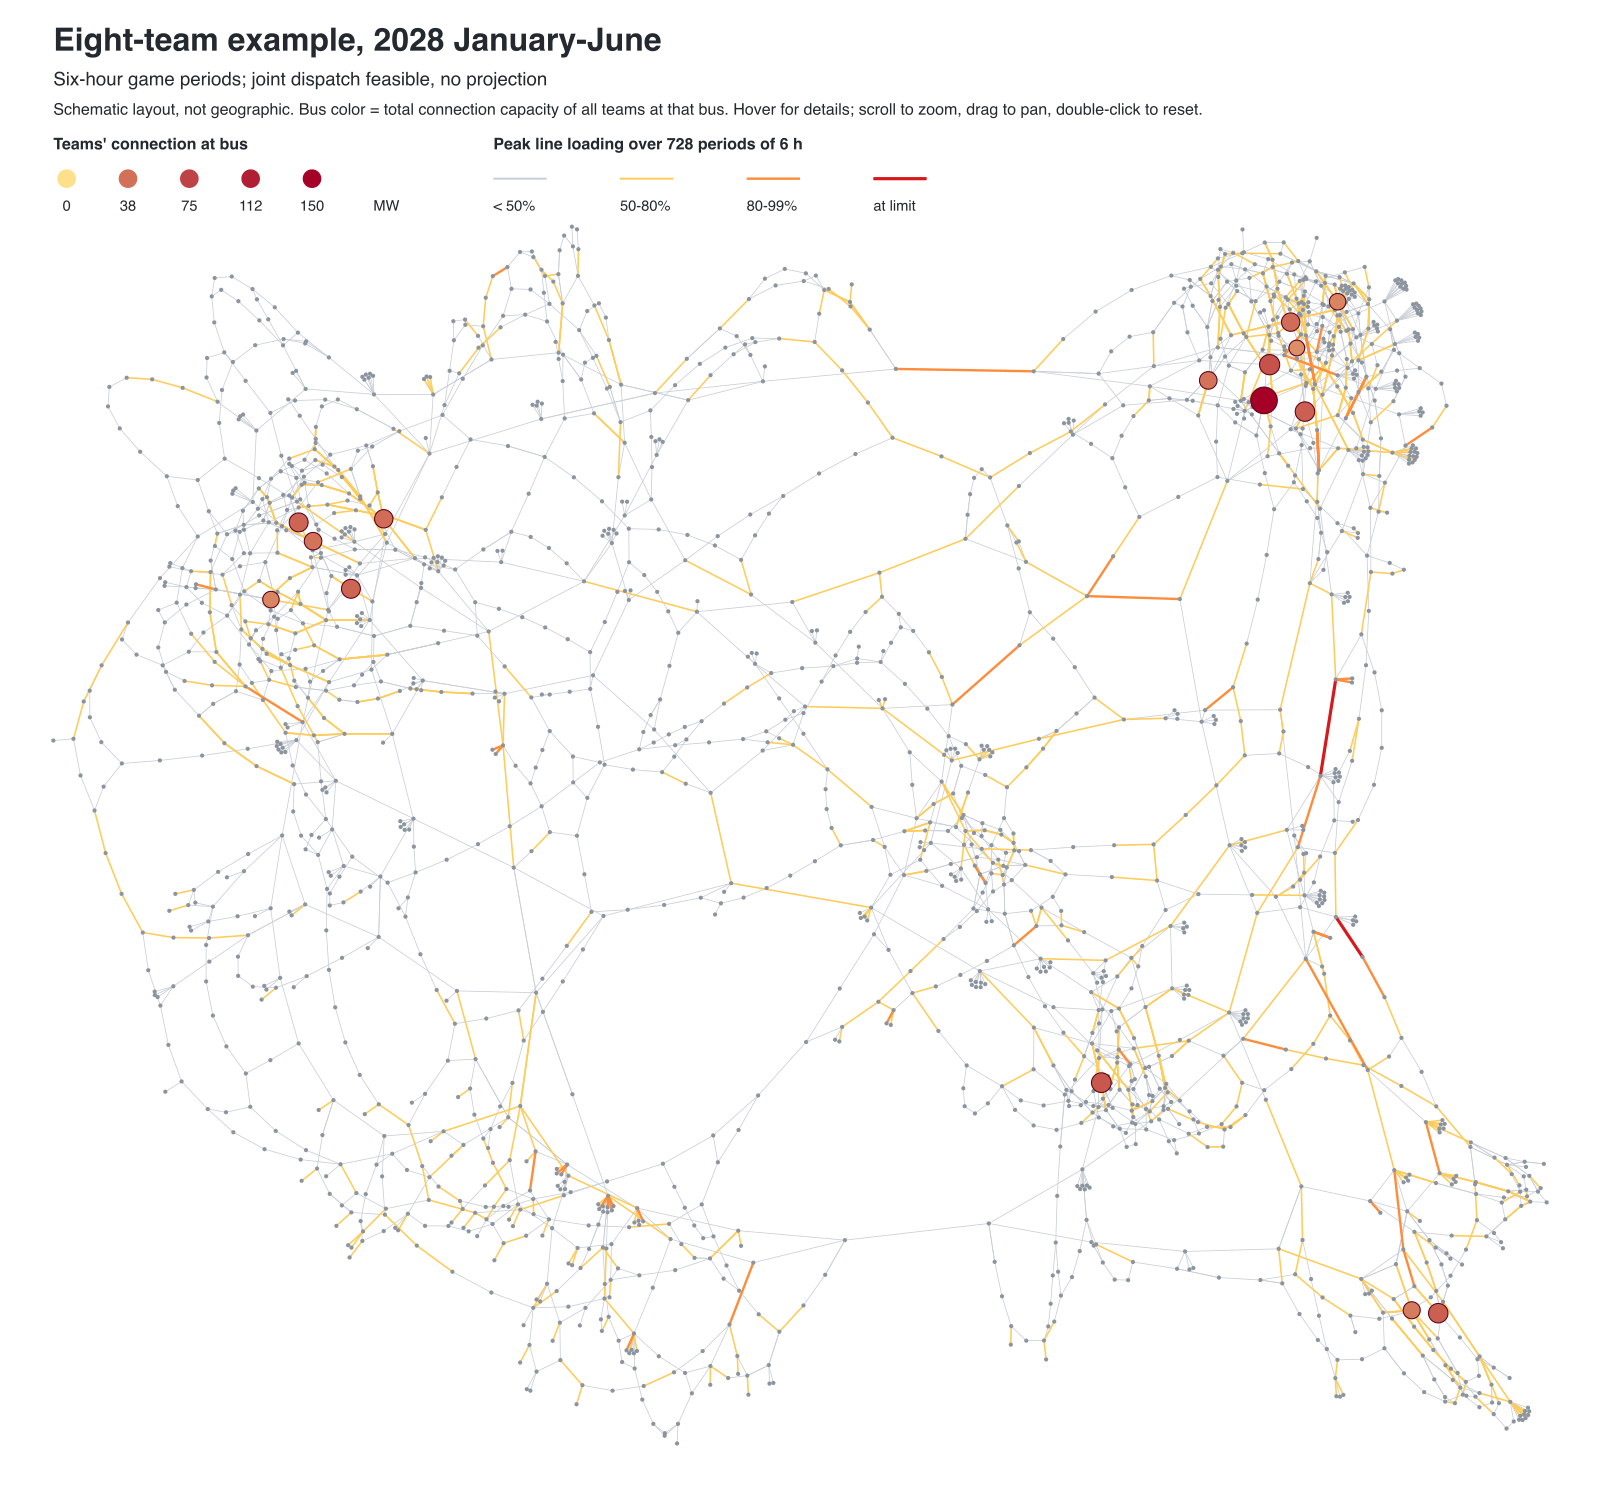
\includegraphics[width=0.92\linewidth]{figures/grid_map.png}\\[-0.2em]
      {\scriptsize Eight-team example: bus color = total MW of all teams; line
      color = peak loading.}
    \end{column}
  \end{columns}
\end{frame}

\begin{frame}{Takeaways}
  \begin{itemize}
    \item Hosting capacity is an LP: the DCOPF with a ``maximize the new load''
      objective.
    \item Time: a constant load is limited by the \alert{worst} period.
      Generation adds $G$; storage moves the limit toward the
      \alert{average}; flexibility toward the $(K{+}1)$-th worst.
    \item Space: single-bus numbers are intercepts of a region and
      \alert{do not add up}.
    \item With many applicants, allocation is a design choice (queue,
      proportional fairness, prices), and it turns planning into a game.
  \end{itemize}
  \vspace{0.6em}
  \textbf{Discussion.} How should a utility allocate scarce headroom among
  data centers? What would you change in the game's projection rule?
\end{frame}

\begin{frame}[allowframebreaks]{References}
  \scriptsize
  \begin{itemize}
    \item M. H. J. Bollen and F. Hassan, \emph{Integration of Distributed Generation in the Power System}, Wiley-IEEE Press, 2011.
    \item M. Bollen and S. R\"onnberg, ``Hosting capacity of the power grid for renewable electricity production and new large consumption equipment,'' \emph{Energies} 10(9):1325, 2017.
    \item M. Rylander, L. Rogers, J. Smith, ``Distribution feeder hosting capacity: what matters when planning for DER?'' EPRI 3002004777, 2015.
    \item E. Mulenga, M. H. J. Bollen, N. Etherden, ``A review of hosting capacity quantification methods for photovoltaics in low-voltage distribution grids,'' \emph{IJEPES} 115:105445, 2020.
    \item S. M. Ismael et al., ``State-of-the-art of hosting capacity in modern power systems with distributed generation,'' \emph{Renewable Energy} 130:1002--1020, 2019.
    \item M. Alturki, A. Khodaei, A. Paaso, S. Bahramirad, ``Optimization-based distribution grid hosting capacity calculations,'' \emph{Applied Energy} 219:350--360, 2018.
    \item T. E. C. de Oliveira et al., ``The concept of dynamic hosting capacity for distributed energy resources,'' \emph{Energies} 12(13):2576, 2019.
    \item S. Gong and J. F. G. Cobben, ``Adaptive facet selection in multidimensional hosting capacity region assessment,'' \emph{EPSR} 234:110654, 2024.
    \item P. Cicilio et al., ``Transmission hosting capacity of distributed energy resources,'' \emph{IEEE TSTE} 12(2):794--801, 2021.
    \item H. Wan et al., ``Impact of security modeling fidelity on hyperscale data center hosting capacity assessment,'' arXiv:2610.18405, 2026.
    \item P. Ren, W. Sun, F. Teng, ``Hosting capacity assessment of data centers with voltage ride-through capability in power systems,'' arXiv:2609.03030, 2026.
    \item N. Etherden and M. H. J. Bollen, ``Increasing the hosting capacity of distribution networks by curtailment of renewable energy resources,'' IEEE PowerTech, 2011.
    \item L. H. Macedo et al., ``Increasing the hosting capacity for renewable energy in distribution networks,'' IEEE ISGT, 2017.
    \item N. Gu, G. Chen, J. Qin, ``The role of flexible connection in accelerating load interconnection in distribution networks,'' HICSS 2026, arXiv:2510.11476.
    \item N. Gu, V. Kekatos, J. Qin, ``Flexible connection to accelerate load interconnection in partially measured distribution grids,'' ACM e-Energy 2026.
    \item G. C. Sarker and N. Dahlin, ``Risk-aware hosting capacity analysis for flexible load interconnection in distribution networks,'' arXiv:2604.20185, 2026.
    \item F. P. Kelly, A. K. Maulloo, D. K. H. Tan, ``Rate control for communication networks: shadow prices, proportional fairness and stability,'' \emph{JORS} 49(3):237--252, 1998.
    \item M. Z. Liu et al., ``On the fairness of PV curtailment schemes in residential distribution networks,'' \emph{IEEE TSG} 11(5):4502--4512, 2020.
    \item D. Gebbran et al., ``Fair coordination of distributed energy resources with Volt-Var control and PV curtailment,'' \emph{Applied Energy} 286:116546, 2021.
  \end{itemize}
\end{frame}

\end{document}
